\chapter{实验技术 II：实践中的合成与分析}\label{ch:b2:lab-techniques-2}

周一早晨，一个格氏反应失败了：烧瓶只冲洗过却未干燥，残留的几滴水
在试剂生成的同时便将其破坏。改在烘箱中干燥的玻璃仪器里重做，
在氮气保护下将卤代烃逐滴加入搅拌着的冷却烧瓶中，同一反应
便能成功。化学本身并未改变，改变的是装置。本章讨论的是把纸面上的反应
变为小瓶中产物的实践：控制反应、隔绝空气与水、
后处理、提纯，并证明所得产物。

\begin{omfigure}
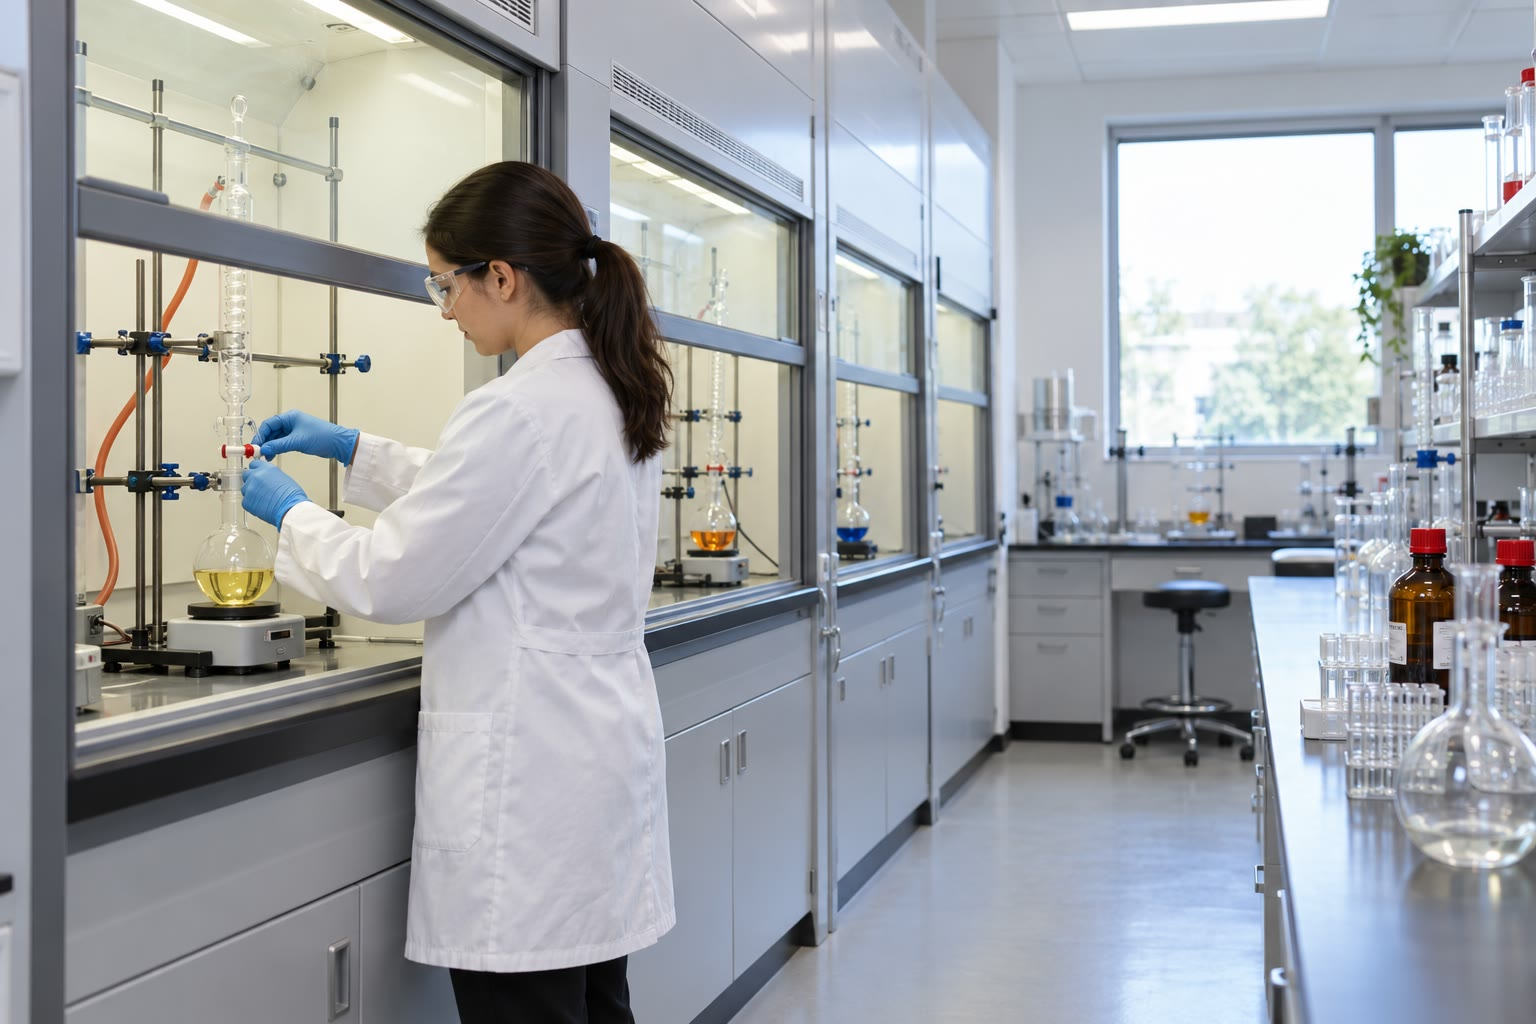
\includegraphics[width=0.56\linewidth]{images/book3/ai/b2-35-synthesis-lab.jpg}

{\small 有机合成实验室：反应在通风橱中进行，烧瓶用夹子固定在支架上
（示意图）。}
\end{omfigure}

\begin{recall}
第 1 册的内容：危害与 GHS 标签、萃取、重结晶、蒸馏、薄层
色谱法与 $R_f$、熔点、格氏试剂。\Cref{ch:b2:reaction-enthalpy}：反应
焓与绝热温升。\cref{ch:b2:chromatography}、
\cref{ch:b2:structure-determination}与\cref{ch:b2:measurement-statistics}：分析。
\end{recall}

\section{控制反应过程}

烧瓶中的反应在发生处释放热量。化学家借助浴槽
（冰水、冰盐混合物，以及获得最低温度时用的干冰丙酮），借助沸腾溶剂的回流
使温度不超过其沸点，同时冷凝器将
蒸气冷凝回流，并通过控制试剂的加入速率。放在液体中而非
浴槽中的内部温度计，才能测得真正关键的温度。

\begin{proposition}[累积]\label{prop:b2:lab-techniques-2:accumulation}
若试剂的加入速率快于其反应速率，则未反应的量 $n_{\mathrm{acc}}$ 会累积。若
此后它一次性全部反应且不加冷却，热容为 $C$ 的混合物温度升高：
\begin{equation*}
\Delta T_{\mathrm{ad}} = \frac{n_{\mathrm{acc}}\,|\Delta_rH|}{C}.
\end{equation*}
\end{proposition}

\begin{proof}
$n_{\mathrm{acc}}$ 的反应在恒压下释放 $n_{\mathrm{acc}}|\Delta_rH|$
（见\cref{ch:b2:reaction-enthalpy}）；无热交换时，其热量全部用于加热混合物，与
绝热火焰温度相同（见\cref{def:b2:reaction-enthalpy:flame-temperature}）：$C\Delta T =
n_{\mathrm{acc}}|\Delta_rH|$。
\end{proof}

格氏试剂的生成常常启动较慢，此时危险最大：卤代烃
在引发之前不断累积，一旦反应终于开始，便会失控。正确做法是先加入少量
，观察反应是否已经开始（升温、变浑浊、缓和回流），再
按冷却能够跟上的速率加入其余部分。

\section{干燥条件与惰性气氛}

\begin{definition}[惰性气氛]\label{def:b2:lab-techniques-2:inert}
反应在\emph{惰性气氛}\index{惰性气氛}中进行，是指装置中的空气
已被不活泼气体（氮气或氩气）置换，并保持略高于大气的压强，使空气
无法进入。
\end{definition}

有机金属试剂、金属氢化物和许多催化剂都会与水和氧气反应。玻璃仪器
需在烘箱中干燥并趁热组装，或在气流下火焰烘烤；溶剂应购买无水溶剂，或
用能与水反应的试剂干燥；液体则用注射器穿过橡胶隔膜转移。
气体经油泡器排出，油泡器既能显示气流，又能防止空气倒流。最敏感的化合物所用的
施伦克线与手套箱，属于第 3 册的内容。

\begin{omfigure}
\begin{tikzpicture}[lab/.style={font=\scriptsize, align=center}]
\fill[omDef!10] (-1.7,-0.3) rectangle (1.7,1.0);
\draw[om glass] (-1.7,1.2) -- (-1.7,-0.3) -- (1.7,-0.3) -- (1.7,1.2);
\foreach \x/\y in {-1.5/0.0,-1.45/0.55,1.3/0.05,1.3/0.6,-1.25/0.3,1.05/-0.15}{
  \draw[omDef!50, fill=white] (\x,\y) rectangle ++(0.18,0.18);}
\pic (f) at (0,0) {threeneck={0.35}{omThm!25}};
\pic[rotate=25] (d) at (f-l) {dropfunnel={0.5}{omMeth!20}};
\pic (c) at (f-c) {condenser};
\pic[rotate=-25] (t) at (0.0,0.42) {thermometer};
\pic (b) at (3.6,3.6) {bubbler};
\draw[thick, black!60] (0,6.25) -- (0,6.75) -- (3.25,6.75) -- (b-in);
\coordinate (dtop) at ($(f-l)+(-1.52,3.26)$);
\draw[thick, black!60] (dtop) -- ++(0,0.35) -- ++(-0.9,0) node[left, lab] {N$_2$};
\node[lab, anchor=north] at (0,-0.4) {冰浴};
\node[lab, anchor=east] at (-1.9,2.6) {加料 \\漏斗};
\node[lab, anchor=west] at (0.55,5.0) {冷凝器};
\node[lab, anchor=west] at (1.75,2.6) {温度计 \\（内部）};
\node[lab, anchor=north] at (3.6,3.45) {油泡器（排气）};
\end{tikzpicture}
\par\vspace{4pt}

{\small 氮气保护下的反应（示意图）。三口烧瓶置于冰浴中，液体中插有内部
温度计；试剂由压力平衡加料漏斗加入，氮气经此漏斗
进入装置，气体经冷凝器与油泡器排出。}
\end{omfigure}

\begin{method}[在氮气保护下建立干燥反应装置]\label{met:b2:lab-techniques-2:anhydrous}
\begin{enumerate}
  \item 在烘箱中干燥玻璃仪器，趁热组装，磨口涂润滑脂或套保护套；装上隔膜
        或加料漏斗、冷凝器和油泡器。
  \item 冷却过程中通氮气置换，全程保持缓慢气流（每一两秒冒一个气泡）。
  \item 固体应在通氮气置换之前加入；干燥溶剂和液体试剂用注射器或套管经
        隔膜加入。
  \item 按计划冷却或加热；先加入少量，确认反应已经开始
        再继续加料。
\end{enumerate}
\end{method}

\section{后处理}

\begin{definition}[后处理]\label{def:b2:lab-techniques-2:work-up}
反应的\emph{后处理}\index{后处理}是指反应结束后，
将反应混合物转变为粗产物的一系列操作：淬灭、萃取与洗涤、干燥、
过滤以及蒸除溶剂。
\end{definition}

\begin{definition}[酸碱萃取]\label{def:b2:lab-techniques-2:acid-base-extraction}
\emph{酸碱萃取}\index{酸碱萃取}是指将溶于有机溶剂中的酸性、碱性和中性有机化合物分离的方法：
用酸或碱的水溶液洗涤该溶液，其中的酸或碱能将一类化合物
转化为离子并进入水中。
\end{definition}

\begin{proposition}[各物质的去向]\label{prop:b2:lab-techniques-2:acid-base-extraction}
碳酸氢钠水溶液（pH 8.3）能萃取羧酸（$\mathrm pK_a$ 约为 4），但不能萃取
酚（$\mathrm pK_a$ 约为 10），萃取酚需用氢氧化钠；稀盐酸能萃取一种胺，
其共轭酸的 $\mathrm pK_a$ 为 4.6 或更大；
中性化合物则留在有机层中。
% ledger: ph:NaHCO3, pka:benzoic, pka:phenol, pka:anilinium
\end{proposition}

\begin{proof}
当 $\mathrm{pH} > \mathrm pK_a$ 时，物种主要以碱式存在，而当
$\mathrm{pH} > \mathrm pK_a + 2$ 时，碱式占比超过 99~\%。在 pH 8.3 时，苯甲酸（4.2）超过 99~\% 为苯甲酸根，
该离子留在水中；苯酚（9.99）约 2~\% 为苯氧负离子（$10^{8.3 - 10.0}$），基本留在
有机层中，中性形式在其中分配。在氢氧化钠溶液（pH 高于 12）中，苯酚
转化为苯氧负离子。在稀盐酸（pH 约为 1）中，苯胺（苯胺正离子 4.6）超过
99~\% 以苯胺正离子形式存在。水相中的每种离子，经反向调节 pH，
即可使其重新生成中性化合物，再将其萃取出来。
\end{proof}

\begin{omfigure}
\begin{tikzpicture}[x=1cm, y=1cm, st/.style={draw=black!70, rounded corners=2pt, fill=white,
  font=\scriptsize, align=center, inner sep=3pt, text width=3.0cm}, ar/.style={->, thick, black!70}]
\node[st, fill=omDef!10] (m) at (0,0) {苯甲酸、苯酚、\\苯胺、萘 \\溶于乙醚中};
\node[st, fill=omThm!10] (a1) at (5.0,0) {水相：苯甲酸根 \\$\to$ HCl $\to$ 苯甲酸};
\node[st] (o1) at (0,-1.6) {苯酚、苯胺、\\萘};
\node[st, fill=omThm!10] (a2) at (5.0,-1.6) {水相：苯氧负离子 \\$\to$ HCl $\to$ 苯酚};
\node[st] (o2) at (0,-3.2) {苯胺、萘};
\node[st, fill=omThm!10] (a3) at (5.0,-3.2) {水相：苯胺正离子 \\$\to$ NaOH $\to$ 苯胺};
\node[st, fill=omMeth!10] (o3) at (0,-4.8) {萘 \\（干燥后蒸除溶剂）};
\draw[ar] (m) -- node[above, font=\tiny] {NaHCO$_3$ 洗涤} (a1);
\draw[ar] (m) -- (o1); \draw[ar] (o1) -- node[above, font=\tiny] {NaOH 洗涤} (a2);
\draw[ar] (o1) -- (o2); \draw[ar] (o2) -- node[above, font=\tiny] {HCl 洗涤} (a3);
\draw[ar] (o2) -- (o3);
\pic at (8.6,-3.6) {sepfunnel={omDef!25}{omThm!20}};
\node[font=\scriptsize, align=center] at (8.6,-4.0) {分液漏斗};
\end{tikzpicture}
\par\vspace{4pt}

{\small 四种化合物的酸碱分离（\cref{prop:b2:lab-techniques-2:acid-base-extraction}）。
有机层（左栏）每经一次洗涤便失去一类化合物；右栏的每份水相萃取液
在 pH 反向调节后，可重新得到其中的化合物。}
\end{omfigure}

\begin{definition}[干燥剂]\label{def:b2:lab-techniques-2:drying-agent}
\emph{干燥剂}\index{干燥剂}是一种无水盐，如硫酸镁或硫酸钠，
它以水合方式结合有机溶液中溶解的水，随后
经过滤除去。
\end{definition}

\begin{method}[从反应瓶到粗产物]\label{met:b2:lab-techniques-2:work-up}
\begin{enumerate}
  \item 淬灭：用合适的水溶液破坏剩余的活性试剂，缓慢进行，
        并注意冷却。
  \item 用有机溶剂萃取，分层（滴入一滴水可判断各层归属）；
        再次萃取水层。
  \item 合并有机层并洗涤（依次用酸、碱，然后用盐水，即
        饱和氯化钠溶液，可除去大部分溶解的水）。
  \item 用干燥剂干燥，直至部分干燥剂仍呈自由流动状态；过滤。
  \item 在减压下用旋转蒸发仪蒸除溶剂；称量粗产物。
\end{enumerate}
\end{method}

\section{纯化}

\begin{definition}[快速柱色谱]\label{def:b2:lab-techniques-2:flash}
\emph{快速柱色谱}\index{快速柱色谱}是一种以硅胶为固定相的制备型柱色谱，其中
洗脱剂借助轻微的气压被压过色谱柱，数克物质的分离
只需几分钟；洗脱剂由同种硅胶上的薄层色谱选定。
\end{definition}

\begin{proposition}[柱体积]\label{prop:b2:lab-techniques-2:column-volumes}
在薄层板上比移值为 $R_f$ 的化合物，在同种硅胶与洗脱剂构成的色谱柱中
约经过 $1/R_f$ 个柱体积的洗脱剂后离开色谱柱。
\end{proposition}

\begin{proof}[论证]
在薄层板上，化合物移动的距离是溶剂前沿的 $R_f$ 倍，其平均速率为
洗脱剂的 $R_f$ 倍。在色谱柱中，相同的分配给出相同的速率比，因此
化合物需要充满色谱柱的洗脱剂体积（即死体积）的 $1/R_f$ 倍才能被洗出；
在\cref{ch:b2:chromatography}中，$R_f \approx 1/(1 + k)$。$R_f = 0.25$ 的化合物
约在四个柱体积后流出，与 0.5 的化合物（两个柱体积）充分分离。
\end{proof}

\begin{omfigure}
\begin{tikzpicture}[lab/.style={font=\scriptsize, align=left, anchor=west}]
\pic (k) at (0,0) {chromcolumn={3.4}};
\node[lab] at (0.6,4.6) {洗脱剂};
\node[lab] at (0.6,3.55) {砂};
\node[lab] at (0.6,2.2) {硅胶层};
\foreach \i/\c in {0/white, 1/omThm!25, 2/omThm!25, 3/white, 4/omDef!25, 5/omDef!25, 6/white}{
  \pic at ({2.4+0.55*\i},-1.2) {testtube={0.45}{\c}};}
\node[font=\scriptsize] at (4.05,-1.6) {收集液 1 至 7};
\pic at (7.6,-1.2) {tlcplate};
\foreach \j/\x in {2/7.15,3/7.45,5/7.75,6/8.05}{\node[font=\tiny] at (\x,-1.38) {\j};}
\fill[omThm] (7.45,0.95) circle (0.06); \fill[omThm] (7.15,0.95) circle (0.06);
\fill[omDef] (8.05,-0.05) circle (0.06); \fill[omDef] (7.75,-0.05) circle (0.06);
\node[font=\scriptsize, align=center] at (7.6,2.15) {收集液的 \\薄层色谱};
\end{tikzpicture}
\par\vspace{4pt}

{\small 快速柱色谱（示意）。粗产物加到硅胶顶部后洗脱；
洗脱液分份收集，收集液的薄层色谱板显示各化合物的洗出位置
（此处，快的非极性化合物位于第 2--3 份，慢者位于第 5--6 份），纯净的收集液
予以合并。}
\end{omfigure}

\begin{method}[快速柱色谱操作]\label{met:b2:lab-techniques-2:flash}
\begin{enumerate}
  \item 用薄层色谱选择洗脱剂：目标化合物的 $R_f$ 约为 0.25--0.35，尽量远离
        杂质。
  \item 装柱时，硅胶质量约为粗产物质量的 30 至 100 倍，可用浆料法或干法装填；在上方加入一层
        砂。
  \item 用尽量少的溶剂溶解粗产物后上样（或使其吸附在少量硅胶上）。
  \item 稍加压力洗脱，收集馏分，用薄层色谱检测，合并纯净的馏分
        后蒸去溶剂。
\end{enumerate}
\end{method}

液体若在沸点附近分解，则采用减压蒸馏，
此时其沸点降低。

\begin{definition}[减压蒸馏]\label{def:b2:lab-techniques-2:reduced-pressure}
称\emph{减压蒸馏}\index{减压蒸馏}为在通过压力计与真空泵相连的装置中进行的，
所用压强使液体
在其能承受的温度下沸腾的蒸馏。
\end{definition}

\begin{proposition}[减压下的沸腾]\label{prop:b2:lab-techniques-2:reduced-pressure}
设 $T_b$ 为参考压强 $p^\circ$ 下的沸点，并将 $\Delta_{\mathrm{vap}}H$
视为常数，则压强为 $p$ 时的沸点由下式给出
\begin{equation*}
\frac{1}{T} = \frac{1}{T_b} - \frac{R}{\Delta_{\mathrm{vap}}H}\ln\frac{p}{p^\circ}.
\end{equation*}
\end{proposition}

\begin{proof}
液体在其蒸气压等于上方压强时沸腾。物理学中的克劳修斯–克拉珀龙关系式
$\mathrm d\ln p/\mathrm dT = \Delta_{\mathrm{vap}}H/(RT^2)$，适用于理想蒸气且
液体体积可忽略的情形，在 $(T_b, p^\circ)$ 与 $(T, p)$ 之间积分，得 $\ln(p/p^\circ) =
-(\Delta_{\mathrm{vap}}H/R)(1/T - 1/T_b)$；整理即得结论。
\end{proof}

\begin{omfigure}
\begin{tikzpicture}
\begin{axis}[width=0.72\linewidth, height=5.2cm, xmode=log, xmin=5, xmax=1100, ymin=0, ymax=190,
  xlabel={压强 (\unit{mbar})}, ylabel={沸点 (\unit{\degreeCelsius})},
  label style={font=\small}, tick label style={font=\scriptsize}, grid=major, grid style={black!10},
  legend style={font=\scriptsize, at={(0.02,0.98)}, anchor=north west}, legend cell align=left]
\addplot[omDef, thick] table[x=p, y=bromobenzene] {figdata/out/bachelor-2-vacuum-boiling.dat};
\addplot[omThm, thick] table[x=p, y=benzaldehyde] {figdata/out/bachelor-2-vacuum-boiling.dat};
\addplot[only marks, mark=o, mark size=2pt, omDef] coordinates {(7,27.75)};
\addplot[only marks, mark=o, mark size=2pt, omThm] coordinates {(13,61.85)};
\legend{溴苯, 苯甲醛, 实测}
\end{axis}
\end{tikzpicture}

{\small 沸点随压强的变化（见\cref{prop:b2:lab-techniques-2:reduced-pressure}），
其中汽化焓与沸点取自 NIST WebBook。圆圈为实测的
沸点，分别位于 7 与 \qty{13}{mbar}，未用于曲线拟合：简单公式的误差在几开尔文以内。
将压强从 1 bar 降至 \qty{20}{mbar}，沸点降低超过
\qty{100}{K}。}
% figdata: bachelor-2/vacuum-boiling.py
% ledger: tb:bromobenzene, dvap:bromobenzene, tbp:bromobenzene.7mbar, tb:benzaldehyde, dvap:benzaldehyde, tbp:benzaldehyde.13mbar
\end{omfigure}

\section{纯度与鉴定}

通过将产物的谱图和物理常数与预期化合物的进行比较来鉴定产物
（见\cref{ch:b2:structure-determination}）；其纯度需另行测定，因为产物
可能是正确的化合物，却仍含有百分之几的其他物质。

\begin{method}[报告纯度与产率]\label{met:b2:lab-techniques-2:purity}
\begin{enumerate}
  \item 检查固体的熔程（纯净化合物的熔程应窄，且接近文献值），
        并用两种洗脱剂检查其薄层色谱（应仅呈一个斑点）。
  \item 测定纯度：可用气相色谱或高效液相色谱的面积百分数（除非已知响应因子，否则仅为估计值，
        见\cref{ch:b2:chromatography}），或采用定量核磁共振氢谱，将产物的积分
        与每种杂质的积分相比较，或与称量的内标相比较。
  \item 换算为所分离物质中产物的质量分数 $w$。
  \item 以纯度校正后的产率报告：$\rho = w\,m/(n_{\mathrm{lim}}M)$，其中 $m$ 为
        分离所得质量，$n_{\mathrm{lim}}$ 为限量反应物的物质的量，$M$ 为摩尔质量。
\end{enumerate}
\end{method}

对于具有旋光性的产物，比旋光度可用于检验其立体化学纯度；
对映体过量及其测定将在本科三年级分册中讨论。

\begin{safety}{\ghs[5mm]{GHS02}\,\ghs[5mm]{GHS06}\,\ghs[5mm]{GHS07}\,\ghs[5mm]{GHS08}\,\ghs[5mm]{GHS09}}
乙醚和四氢呋喃极易燃，储存时会形成爆炸性过氧化物；
实验室内禁止明火，蒸馏前须检验旧瓶。溴苯易燃，且对水生生物有毒；
镁屑易燃。真空玻璃仪器须检查有无星形裂纹，并加以防护。
% ledger: ghs:ether, ghs:THF, ghs:bromobenzene, ghs:Mg, ghs:MgSO4
\end{safety}

\section{练习}

\begin{exercise}[$\star$]\label{exo:b2:lab-techniques-2:1}
对于需在约 \qty{0}{\degreeCelsius}、约
\qty{-15}{\degreeCelsius} 和 \qty{-78}{\degreeCelsius} 下进行的反应，各应选用哪种冷浴？
\end{exercise}

\begin{exercise}[$\star$]\label{exo:b2:lab-techniques-2:2}
一次萃取使用密度大于水的二氯甲烷。哪一层为有机相？如何检验？
\end{exercise}

\begin{exercise}[$\star$]\label{exo:b2:lab-techniques-2:3}
如何判断乙醚溶液中已加入足量的硫酸镁？
\end{exercise}

\begin{exercise}[$\star$]\label{exo:b2:lab-techniques-2:4}
在 4\,:\,1 的己烷–乙酸乙酯中，某产物的 $R_f = 0.65$，杂质为 0.75。
若用于装柱，应改变哪一项，并朝哪个方向改变？
\end{exercise}

\begin{exercise}[$\star\star$]\label{exo:b2:lab-techniques-2:5}
给出从乙醚
溶液中分离苯甲酸、苯酚、苯胺和萘所需洗涤的顺序，并以各化合物的 $\mathrm pK_a$ 说明每一步的依据，以及各化合物如何回收。
\end{exercise}

\begin{exercise}[$\star\star$]\label{exo:b2:lab-techniques-2:6}
估算溴苯和苯甲醛在 \qty{20}{mbar} 下的沸点。
\end{exercise}

\begin{exercise}[$\star\star$]\label{exo:b2:lab-techniques-2:7}
加成过程中，已有 \qty{0.050}{mol} 的试剂未反应而累积。取 $\Delta_rH =
\qty{-200}{kJ/mol}$，混合物热容为 \qty{400}{J/K}（习题数据），
可能出现多大的温升？
\end{exercise}

\begin{exercise}[$\star\star$]\label{exo:b2:lab-techniques-2:8}
高效液相色谱图显示产物占总峰面积的 96.0~\%。为何这尚不能说明质量纯度？
同一样品的质子谱中，产物单峰（1H）积分为 1.00，杂质单峰
（3H）积分为 0.12；产物 \qty{200}{g/mol}，杂质 \qty{100}{g/mol}（习题数据）。计算
产物的质量分数。
\end{exercise}

\begin{exercise}[$\star\star$]\label{exo:b2:lab-techniques-2:9}
\qty{4.10}{g} 产物（\qty{164}{g/mol}，质量纯度 95.0~\%）由 \qty{0.0300}{mol}
限量反应物得到。分别计算未校正和经纯度校正的产率。
\end{exercise}

\begin{exercise}[$\star\star\star$]\label{exo:b2:lab-techniques-2:10}
格氏反应在加入醛后得到苯，而几乎没有醇。列出
可能的原因，并说明各自如何避免。
\end{exercise}

\begin{exercise}[$\star\star\star$]\label{exo:b2:lab-techniques-2:11}
放大规模时，\qty{1.00}{mol} 卤代物与 $\Delta_rH = \qty{-270}{kJ/mol}$ 反应，所用反应器
的冷却至多移走 \qty{150}{W}（习题数据）。最短的安全滴加时间是多少？
若滴加更快，会发生什么？
\end{exercise}

\begin{exercise}[$\star\star\star$]\label{exo:b2:lab-techniques-2:12}
粗固体 \qty{13.0}{g} 可用重结晶提纯（一步，回收率 80~\%，纯度
99~\%），或用快速柱色谱提纯（回收率 95~\%，纯度 99.5~\%，溶剂 \qty{1.5}{L}）（习题
数据）。比较两种路线。
\end{exercise}

\section{问题：规范的格氏反应}

\begin{problem}[{周末问题 --- 危害与干燥装置、受控加料及
积累危险、后处理、快速柱色谱提纯及纯度校正产率}]
\label{pb:b2:lab-techniques-2:1}
习题数据。溴化苯基镁由 \qty{15.7}{g} 溴苯与 \qty{2.67}{g} 镁屑
在干燥的乙醚中制得，然后加入 \qty{9.55}{g} 苯甲醛；后处理
用氯化铵水溶液处理，得到二苯甲醇。试剂生成的反应焓：$\Delta_rH =
\qty{-270}{kJ/mol}$；混合物热容 \qty{170}{J/K}；起始温度 \qty{20}{\degreeCelsius}。薄层色谱
（9\,:\,1 己烷–乙酸乙酯）：联苯 $R_f = 0.85$，二苯甲醇 0.25。经柱分离后，
得 \qty{12.50}{g}。该物质的质子核磁共振：\ce{CH(OH)} 单峰（1H）积分为 1.00，芳香区
积分为 10.90。摩尔质量（\unit{g/mol}）：溴苯 157.01，苯甲醛 106.12，二苯甲醇
184.24，联苯 154.21；Mg 24.305。
% ledger: ghs:ether, ghs:bromobenzene, ghs:Mg, ghs:benzaldehyde, ghs:NH4Cl, ghs:biphenyl, ghs:benzhydrol, tb:ether, aw:Mg, aw:C, aw:H, aw:Br, aw:O, nmr:biphenyl

\medskip
\noindent\textbf{第一部分 --- 危害与装置。}
\begin{enumerate}
  \item 给出乙醚、溴苯和镁的主要危害。
  \item 写出溴化苯基镁与水的反应，并说明为何要用烘干的玻璃仪器。
  \item 为何要在氮气中操作？
  \item 鼓泡器显示什么？它防止什么？
  \item 为何乙醚在此是良好的溶剂？
  \item 计算溴苯和镁的物质的量。哪一种过量？
\end{enumerate}

\medskip
\noindent\textbf{第二部分 --- 受控加料。}
\begin{enumerate}[resume]
  \item 试剂完全生成时释放多少热？
  \item 为何溴苯要逐滴加入？
  \item 反应开始缓慢，在其开始前已加入 20~\% 的溴苯。此时
        可能一次性释放多少热？
  \item 计算绝热温升。
  \item 比较终温与乙醚的沸点，会发生什么？
  \item 应当如何进行加料？
\end{enumerate}

\medskip
\noindent\textbf{第三部分 --- 加成与后处理。}
\begin{enumerate}[resume]
  \item 写出与苯甲醛的反应，并确定限量反应物。
  \item 为何用氯化铵而非强酸淬灭？
  \item 分液漏斗中哪一层是有机相？
  \item 饱和食盐水洗涤的作用是什么？
  \item 溶液如何干燥，溶剂如何除去？
  \item 联苯是主要副产物。它如何生成，什么有利于它的生成？
\end{enumerate}

\medskip
\noindent\textbf{第四部分 --- 提纯与纯度。}
\begin{enumerate}[resume]
  \item 哪种化合物先流出柱子？
  \item 各组分在多少个柱体积后流出？
  \item 由核磁积分，计算分离所得物质中联苯与醇的
        摩尔比。
  \item 计算二苯甲醇的质量分数。
  \item 计算纯二苯甲醇的质量。
  \item 计算理论质量。
  \item 计算未经纯度校正的产率。
  \item 给出经纯度校正后的产率。
\end{enumerate}
\end{problem}
